\documentclass[./\jobname.tex]{subfiles}
\begin{document}
%
% The mode of interfacing the closed loop control and the state machine shall be explained briefly.
% The quality of the control shall be documented.
%
\chapter{Reglerimplementierung und Verifizierung}
%\chapter{Closed Loop Control}
%
\section{Reglermodell}
%
In \autoref{Motor.pdf} ist das Modell des implementierten Motors und des PI-Reglers dargestellt. Das Subsystem ist hierbei der PI-Regler, der als diskreter Regler ausgeführt wurde. Das Subsystem wird mittels Simulink in C-Code übersetzt, der direkt für VxWorks verwendet werden kann. Der Eingangsparameter ist die Istgeschwindigkeit und der Ausgangsparameter die Stellgröße (Motorspannung). Jedoch wurde der generierte C-Code von uns auf C++ portiert und der Zeitgeber von einer asynchron laufenden Clock auf einen Softwarewatchdog programmiert. Dies hat den Vorteil, dass das Anwenderprogramm und der Controller synchron gekoppelt sind.
%
\begin{figure}[H]
	\centering
	\noindent\adjustbox{max width=\textwidth}{%falls größer als \textwidth, wird das Bild verkleinert
		%trim option's parameter order: left bottom right top
		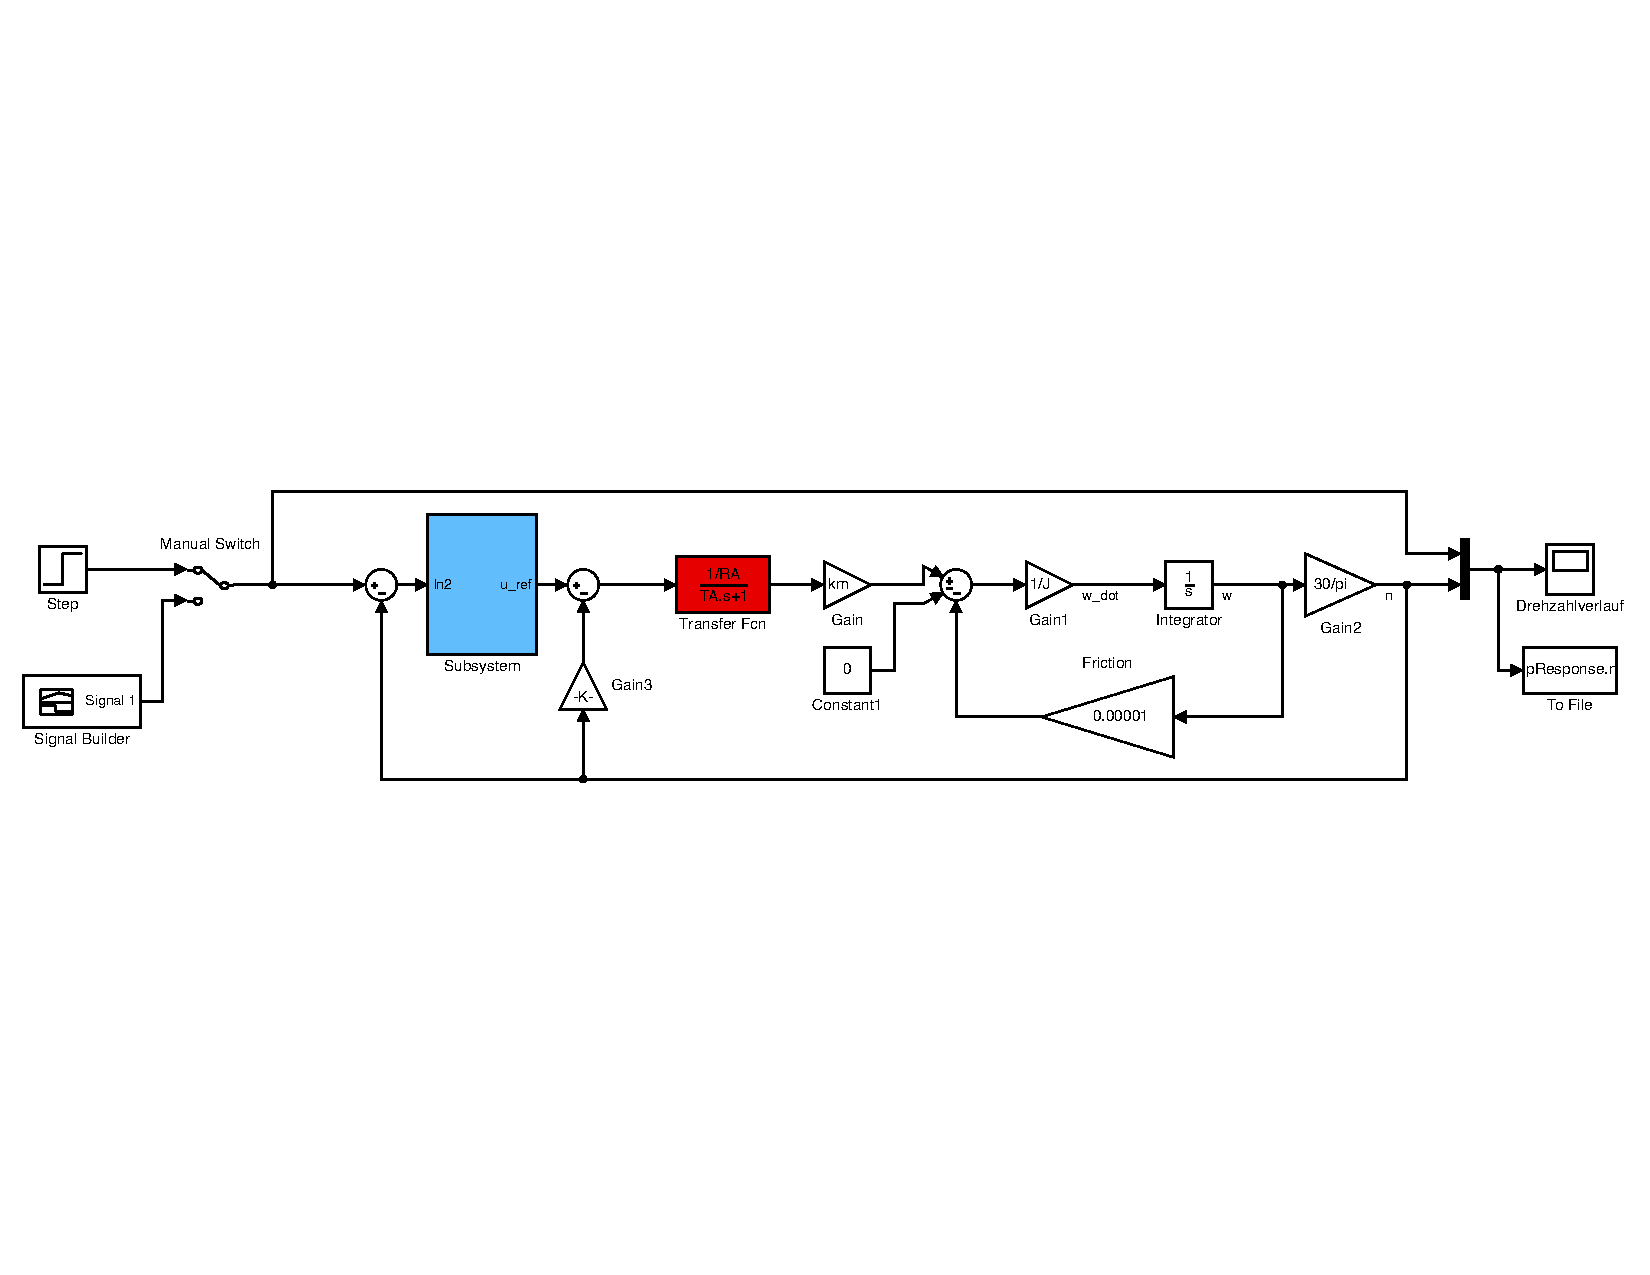
\includegraphics[width=1\textwidth]{./img/4_controller/Motor.pdf}
	}
	\unterschrift{Motormodell}{Eigene Ausarbeitung}{}
	\label{Motor.pdf}
\end{figure}
%
%
Die Drehzahl als Eingangsgröße wird von der Klasse Motor via Membermethode \enquote{getActSpeed()} zur Verfügung gestellt. Die Klasse \enquote{Motor} ruft wiederum eine Membermethode der Klasse \enquote{Encoder} auf. Die \enquote{Encoder} Klasse implementiert die Logik für die Auswertung der Drehzahl. \cref{eq: drehzahl eingang} gibt die implementierte Logik an. Der Faktor \(10^{6}\) kommt von der Auflösung des Zählers. Dieser zählt in \(\mu\)-Schritten, aber die Winkelgeschwindigkeit wird in Sekunden benötigt.
%
\begin{align}
\omega&=\frac{1}{\text{Auflösung Encoder}} \cdot 60~s \cdot10^{6} \frac{1}{x}\label{eq: drehzahl eingang}\\
\omega&= \frac{1.0 }{64.0} \cdot 60.0 \cdot 10^{6} \cdot \frac{1}{x}\\
x &\ldots \text{gefilterter Wert}
\end{align}
%
Der gefilterte Wert wird von der Klasse \enquote{Kalman} zur Verfügung gestellt. Für die Implementierung des Kalman Filters sei auf \autoref{sec:kalmann implementation} verwiesen.\par
%
Mit \cref{eq: ausgangsgleichung} wird die Sollgröße, die vom PI-Regler berechnet wurde, auf den DC-Wandler umgerechnet.
%
\begin{align}
u_{out} &= \frac{\text{Auflösung}}{2.0}\cdot\frac{1}{\text{max. Ausgangsspannug}} \cdot U_{soll}\label{eq: ausgangsgleichung}\\
u_{out} &= \frac{4095.0}{2.0}\cdot\frac{1}{12.0~V} \cdot U_{soll}\\
U_{soll}&\ldots\text{vom Regler berechnete Ausgangspannung}
\end{align}
%
Der Wert \(u_{out}\) wird mittels der Membermethode \enquote{setActSpeed()} und \enquote{drive()} von der \enquote{Motor} Klasse übergeben und diese ist dann zuständig, den gewünschten Wert auf den Ausgang zu schreiben.
%
\section{Reglerkoppelung mit der Statemachine}
%
Der Regler ist eine eigenständige Klasse, die folgende Membermethoden zur Verfügung stellt, um den Verlauf der Rampe zu steuern.
%
\begin{itemize}
	\item \enquote{setProfile()}:Setzt die Beschleunigung und Verzögerungswerte und maximale Geschwindigkeit.
	\item \enquote{setRampUp()}: Es soll bis zur maximalen Geschwindigkeit beschleunigt werden.
	\item \enquote{setRampDown()}: Es soll bis zum Stillstand verzögert werden.
	\item \enquote{setConstantVelocity()}: Es soll eine konstante Geschwindigkeit gefahren werden.
	\item \enquote{setSpeedToZero()}: Stopp der Bewegung.
\end{itemize}
%
Die Statemachine kann auf diese Membermethoden zugreifen und je nach Zustand die Methoden ausführen.\par
%
Der Controller meldet seinen Zustand über die von der Statemachine zur Verfügung gestellte Methode \enquote{sendEvent()} zurück.
%
\section{Verifizierung}
%
In \autoref{fig: stepresponse_old.pdf} ist die Sprungantwort mit den Regelparametern des Auftraggebers abgebildet. Sie enthält den Vorgabewert (\enquote{Step}), die simulierte (\enquote{Stepresponse Simulink}) und zwei gemessene Sprungantworten (\enquote{Stepresponse gemessen}, \enquote{Stepresponse gemessen neu}). Die blaue Kurve ist die Sprungantwort, die ohne Kalmanfilter und mit den gemittelten Zählerwerten aufgenommen wurde. Es ist ersichtlich, dass die Auflösung sehr schlecht ist. Dagegen stimmt die violette Kurve, die mit dem Kalmanfilter und der Zeitdifferenz des Zählers aufgenommen wurde, mit der Wirklichkeit sehr gut überein. Die Risetime \(T_{s}\) und die Ausregelzeiten \(T_{r}\) sind bei beiden nahezu dieselben und liegen weit über den in \autoref{sec: regelguete} definierten Werten.
%
\begin{figure}[H]
	\centering
	\noindent\adjustbox{max width=\textwidth}{%falls größer als \textwidth, wird das Bild verkleinert
		%trim option's parameter order: left bottom right top
		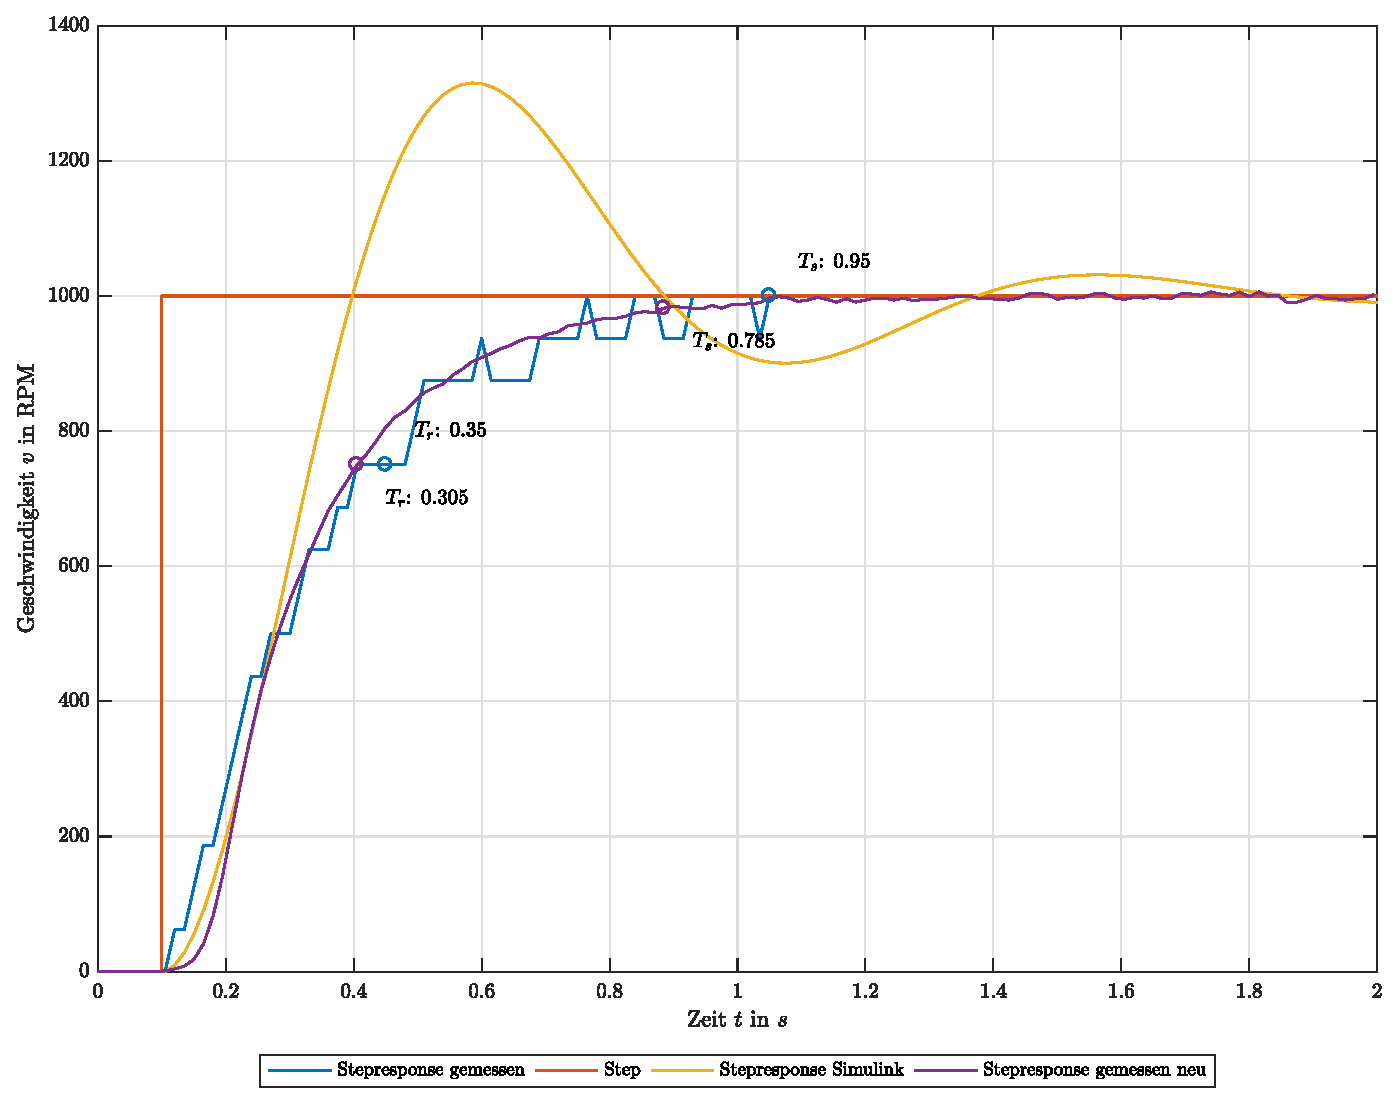
\includegraphics[width=1\textwidth]{./img/4_controller/stepresponse_old.eps}
	}
	\unterschrift{Closed Loop Stepresponse mit Reglerparametern vom Auftraggeber}{Eigene Ausarbeitung}{}
	\label{fig: stepresponse_old.pdf}
\end{figure}
%
Aus diesem Grund wurden eigene Regelparameter verwendet, die in \autoref{fig: stepresponse_new.pdf} dargestellt sind. In \autoref{tab: regler parameter} sind die verwendeten Reglerparameter festgehalten.\par
%
\(K_{p,n}\) gibt die Verstärkung des P-Reglers und \(K_{i,n}\) die des I-Reglers an. \(t_{s,n}\) ist die Zykluszeit, mit der der diskrete Regler arbeitet.
%
\begin{table}[H]
\centering
\begin{tabular}{|c|c|c|}\hline 
			& Standarwerte  & Neue Werte \\ \hline 
\(K_{p,n}\)	& \(8.0 \cdot 10^{-6}\) & \(0.00048\)\\ \hline 
\(K_{i,n}\)	& \(0.015625\) & \(0.0351\)\\ \hline 
\(t_{s,n}\)	& \(0.015625\) &\( 0.015\)\\ \hline 
\end{tabular} 
\unterschrift{Regler Parameter}{Eigene Ausarbeitung}{}
\label{tab: regler parameter}
\end{table}
%
%
Es ist zu erkennen, dass sich die Risetime \(T_{r}\) und ebenfalls die Ausregelzeit \(T_{s}\) halbiert haben. Das Überschwingen beträgt ca. \(2~\%\). Es können jedoch nicht alle Werte, die in \autoref{sec: regelguete} definiert wurden, erreicht werden. Die Gründe liegen bei der zusätzlichen Last, die in Form eines Aluminiumrades an den Motor angeflanscht ist und an der geringen Encoderauflösung sowie an der Zyklusdauer des Reglers.
%
\begin{figure}[H]
	\centering
	\noindent\adjustbox{max width=\textwidth}{%falls größer als \textwidth, wird das Bild verkleinert
		%trim option's parameter order: left bottom right top
		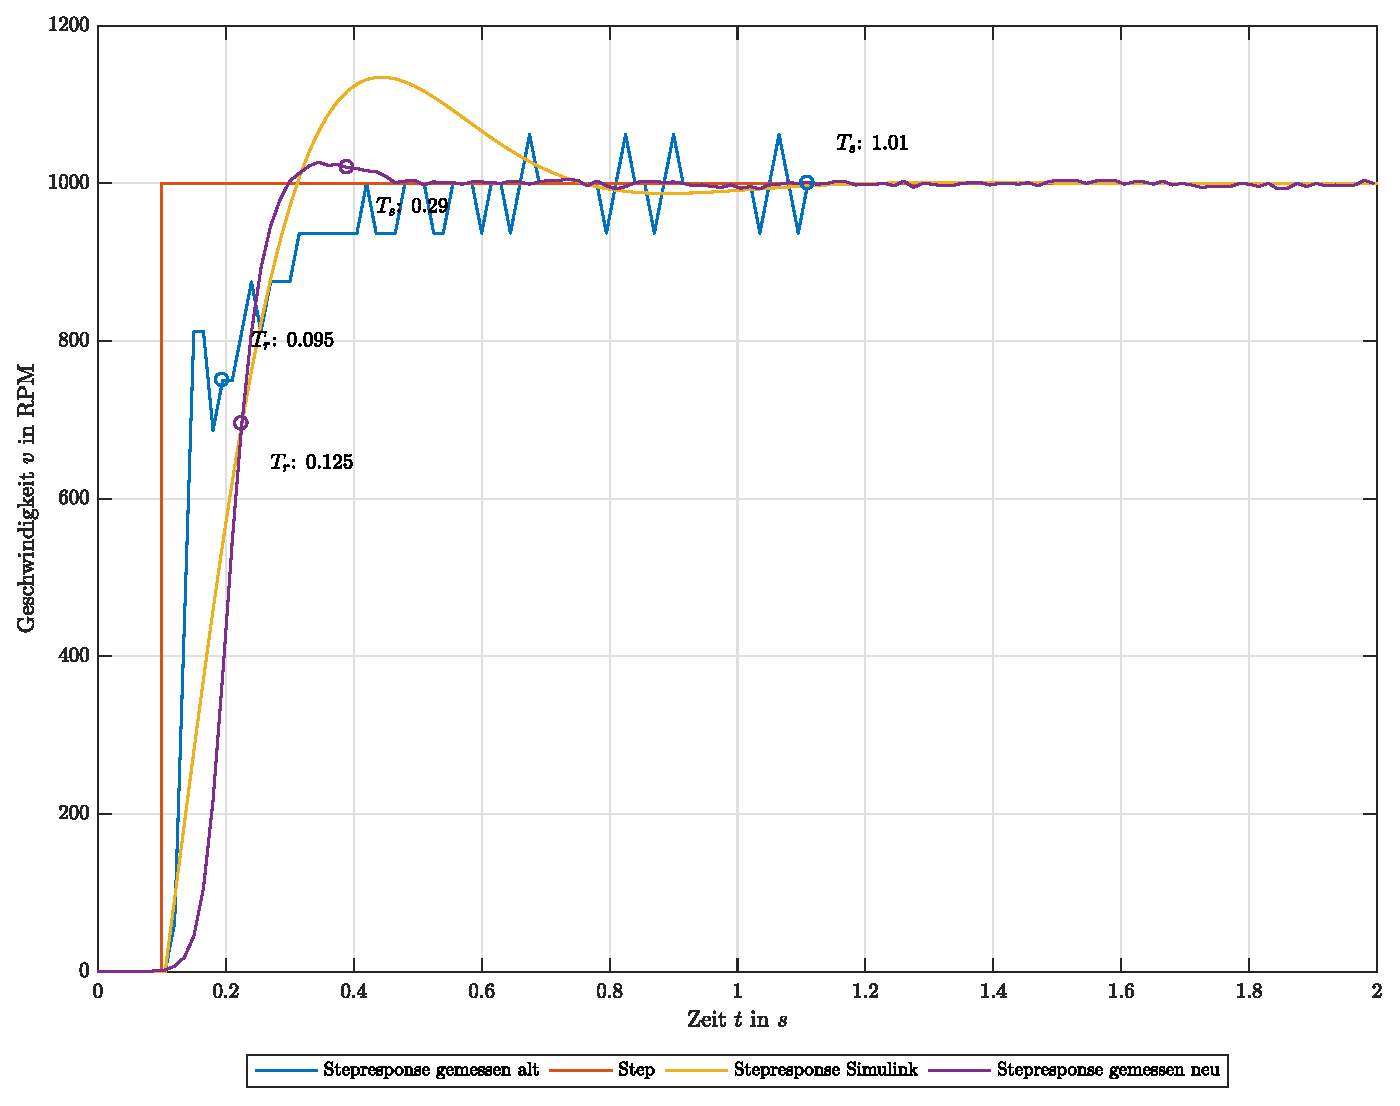
\includegraphics[width=1\textwidth]{./img/4_controller/stepresponse_new.eps}
	}
	\unterschrift{Closed Loop Stepresponse mit eigenen Reglerparametern}{Eigene Ausarbeitung}{}
	\label{fig: stepresponse_new.pdf}
\end{figure}
%
In \autoref{fig: rampresponse.eps} ist die Rampe, die im \modeA und \modeB gefahren wird, abgebildet. Die \enquote{Rampe soll} Kurve gibt das Profil vor, dem der Regler folgen soll. Die \enquote{Rampe ist alt} stellt die gemessene Drehzahl mit den vom Auftraggeber zur Verfügung gestellten Parametern dar. Im Vergleich dazu ist die \enquote{Rampe ist neu} mit den neuen Regelparametern um das Doppelte schneller. Der Grund für die Abweichung beim Beschleunigen, wird auf das Fehlen des Massenträgheitsmomentes im Modell zurück geführt. Das Minimum und das Maximum liegt bei beiden bei ca. \(1818~U/min\) und \(1787~U/min\).
%
\begin{figure}[H]
	\centering
	\noindent\adjustbox{max width=\textwidth}{%falls größer als \textwidth, wird das Bild verkleinert
		%trim option's parameter order: left bottom right top
		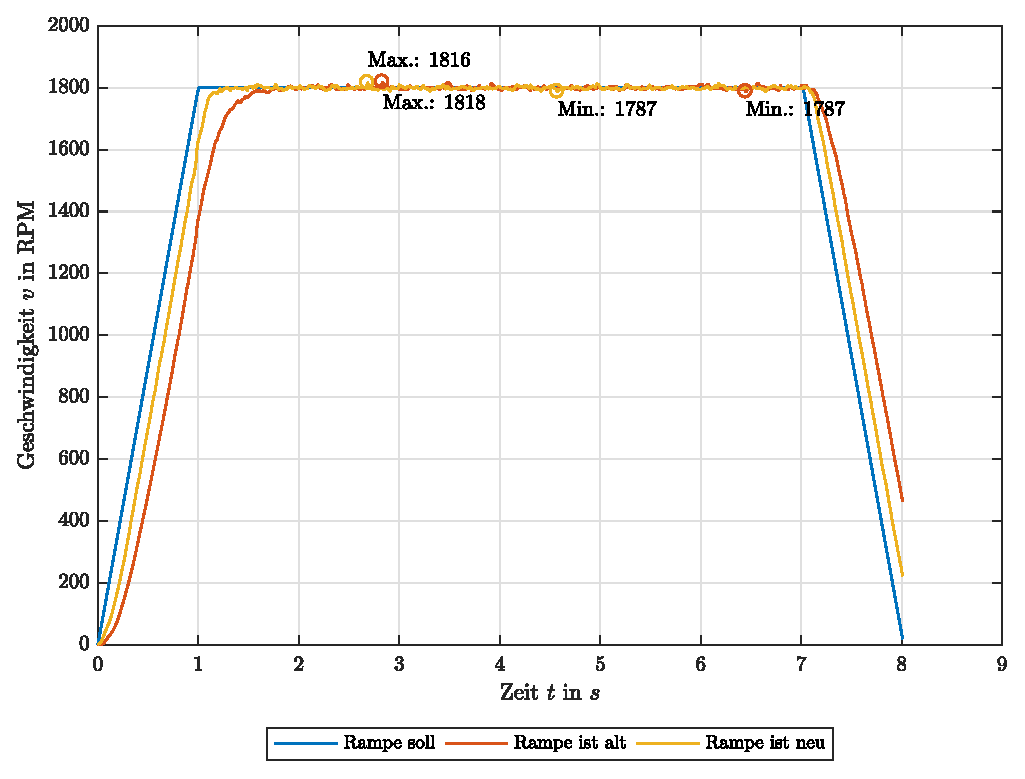
\includegraphics[width=1\textwidth]{./img/4_controller/rampresponse.eps}
	}
	\unterschrift{Rampe Soll Ist Verlgeich}{Eigene Ausarbeitung}{}
	\label{fig: rampresponse.eps}
\end{figure}
%
Um die Differenz zwischen \enquote{Rampe soll} und \enquote{Rampe ist neu} zu minimieren, wurden die Beschleunigungs- und Verzögerungswerte so angepasst, dass ein Verzögern bis auf Stillstand möglich ist. Die vom Auftraggeber vorgegebenen Werte werden hierbei nicht verletzt. Das Ergebnis ist in \autoref{fig: rampresponseNew.eps} dargestellt.
%
\begin{figure}[H]
	\centering
	\noindent\adjustbox{max width=\textwidth}{%falls größer als \textwidth, wird das Bild verkleinert
		%trim option's parameter order: left bottom right top
		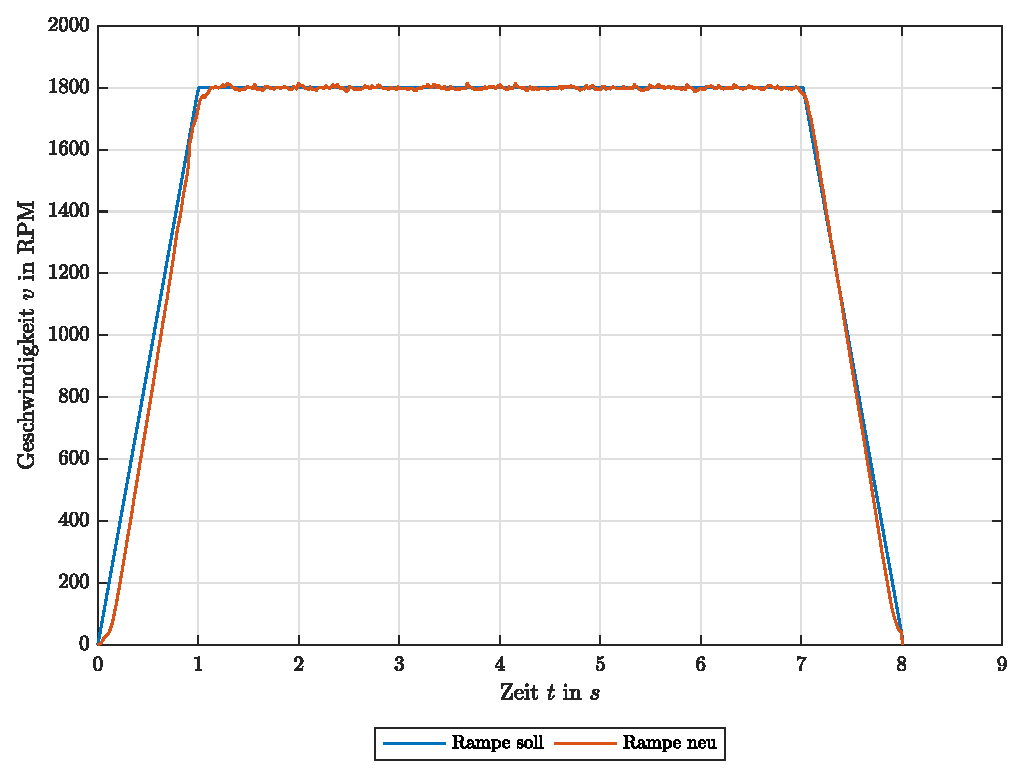
\includegraphics[width=1\textwidth]{./img/4_controller/rampresponseNew.eps}
	}
	\unterschrift{Rampe Soll Ist Verlgeich mit schnellerer Beschleunigung und Verzögerung}{Eigene Ausarbeitung}{}
	\label{fig: rampresponseNew.eps}
\end{figure}
%
\end{document}
